\scanpage{135}
correspondant à des morphismes
\[
\mathcal G'_n\longrightarrow\mathcal G_n
\]
\deleted{\unsure{et|de} \unsure{à} \unsure{l'homo} de \unsure{foncteurs}}
ou encore, composante par composante, à
\[
\varphi_n^\nu:\mathcal G_0\longrightarrow\mathcal G_n\qquad \nu\in[-n,+n]
\]
donné \deleted{par} sur les foncteurs par
\[
\varphi_n^\nu\left(\sum_{i\geq0}a_it^i\right)=t^\nu\sum a_it^i
\]

Ceci posé, on a un

\uline{Th} (i) Le morph. $\unsure{f_n|h_n}:\mathcal G'_n-\mathcal G_n$ est une \uline{immersion fermée surjective}\figure{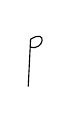
\begin{tikzpicture}[baseline]\draw (0,0)--(.03,.6)..controls(.25,.74)and(.2,.45)..(.03,.5);\end{tikzpicture}}. (ii) Elle induit une immersion ouverte sur $\mathcal G_0\times\{\nu\}$ pour $\nu=\pm n$, mais pour $-n<\nu<+n$, le morphisme induit \uline{n'est pas} une immersion ouverte [même après changement de base quelconque $S\longrightarrow\mathrm{Spec}\,\mathbf Z$, $S\ne\varnothing$]. (iii) Soit $\mathcal G_n^i$ le sous schéma ouvert \inserted{induit} et fermé de $\mathcal G_n$ \deleted{\unsure{image}} par l'image ensembliste $\deleted{\unsure{\varphi_n^i}}\varphi_n(\mathcal G_0\times\{i\})$, où $|i|\leq n$.

\margin{\figure{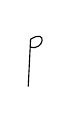
\begin{tikzpicture}[baseline]\draw (0,0)--(.03,.6)..controls(.25,.74)and(.2,.45)..(.03,.5);\end{tikzpicture}} donc $\mathcal G_n$ est réunion disjointe d'ouverts $\mathcal G_n^i$ $(i\in[-n,+n])$, d'ailleurs irréductibles, qui sont les images des $\varphi_n^i$}

Pour $n$ variable, on trouve ainsi un système ``inductif'' \inserted{d'immersions} de préschémas, ayant \unsure{même} \deleted{\unsure{type foncteur}} top. sous-jacent. Donc \unsure{si} $n'\geq n\geq|i|$, le morphisme $\mathcal G_n^i\longrightarrow\mathcal G_{n'}^i$ n'est pas un isomorphisme, et ceci même sur une base $S\ne\varnothing$ quelc.

[Il suffit de regarder sur les corps premiers $\ldots$].
\margin{134}
